\let\negmedspace\undefined
\let\negthickspace\undefined
\documentclass[journal]{IEEEtran}
\usepackage[a5paper, margin=10mm, onecolumn]{geometry}
%\usepackage{lmodern} % Ensure lmodern is loaded for pdflatex
\usepackage{tfrupee} % Include tfrupee package

\setlength{\headheight}{1cm} % Set the height of the header box
\setlength{\headsep}{0mm}     % Set the distance between the header box and the top of the text

\usepackage{gvv-book}
\usepackage{gvv}
\usepackage{cite}
\usepackage{amsmath,amssymb,amsfonts,amsthm}
\usepackage{algorithmic}
\usepackage{graphicx}
\usepackage{textcomp}
\usepackage{xcolor}
\usepackage{txfonts}
\usepackage{listings}
\usepackage{multicol}
\usepackage{enumitem}
\usepackage{mathtools}
\usepackage{gensymb}
\usepackage{comment}
\usepackage[breaklinks=true]{hyperref}
\usepackage{tkz-euclide} 
\usepackage{listings}
% \usepackage{gvv}                                        
\def\inputGnumericTable{}                                 
\usepackage[latin1]{inputenc}                                
\usepackage{color}                                            
\usepackage{array}                                            
\usepackage{longtable}                                       
\usepackage{calc}                                             
\usepackage{multirow}                                         
\usepackage{hhline}                                           
\usepackage{ifthen}                                           
\usepackage{lscape}
\usepackage{tikz}
\usetikzlibrary{patterns}
\usepackage{amsmath}
\usepackage{graphicx}
\usepackage{pgfplots}
\pgfplotsset{compat=1.17} 
\newlength{\mywidth}
\setlength{\mywidth}{0.45\textwidth}    
\begin{document}
\bibliographystyle{IEEEtran}
\vspace{3cm}
\title{2016-CE-'14-26'}
\author{EE24BTECH11023}
%\maketitle
%\newpage
%\bigskip

{\let\newpage\relax\maketitle}

\renewcommand{\thefigure}{\theenumi}
\renewcommand{\thetable}{\theenumi}
\setlength{\intextsep}{10pt} % Space between text and floats


\numberwithin{equation}{enumi}
\numberwithin{figure}{enumi}
\renewcommand{\thetable}{\theenumi}
\begin{enumerate}
    \item The direct runoff hydrograph in response to 5 cm rainfall excess in a catchment is shown in the figure. The area of the catchment (expressed in hectares) is:\\
      \begin{figure}[H]
        \centering
        \begin{tikzpicture}
    \node[below] at (-0.5, -2) {Column};
    \draw[thick,magenta] (-1.5,2.5)--(-1.5,-2);
    \draw[thick,magenta] (0.5,2.5)--(0.5,-2);
    \draw[dashed, thick, brown] (-0.5,2) -- (-0.5,-2);
    \draw[thick] (-2,2) -- (4,2) -- (4,-1) -- (0.4,-2);
    \coordinate (A) at (-1.5,2.5);
    \coordinate (B) at (0.5,2.5);
    \draw[magenta, thick] (-0.834, 2.5) arc[start angle=0, end angle=180, radius=0.333cm];
    \draw[magenta, thick] (-0.834, 2.5) arc[start angle=-180, end angle=0, radius=0.333cm];
    \draw[magenta, thick] (0.498, 2.5) arc[start angle=0, end angle=180, radius=0.333cm];
    \draw[magenta, thick] (-1.5, -2) arc[start angle=-180, end angle=0, radius=0.333cm];
    \draw[magenta, thick] (-0.168, -2) arc[start angle=0, end angle=180, radius=0.333cm];
    \draw[magenta, thick] (-0.168, -2) arc[start angle=-180, end angle=0, radius=0.333cm];
    \draw[thick, red, ->] (3.5,2.5) -- ++(0,-0.5);
    \node[right] at (3.5,2.5) {$P$};
    \draw[<->, thin] (-0.5,2.3) -- node[above] {$e$} ++(4,0);
    \filldraw[red] (-0.5,0.75) circle (2pt) node[left] {$U$};
    \filldraw[red] (-0.5,-0.75) circle (2pt) node[left] {$V$};
    \draw[<->, thin] (-0.75,0.75) -- node[left] {$2a$} ++(0,-1.5);
    \node at (2,0) {Bracket};
\end{tikzpicture}
 
    \end{figure}
    \item The type of flood routing (Group I) and the equation(s) used for the purpose (Group II) are given below:
    \begin{multicols}{2}
        \begin{enumerate}
            \item \underline{Group I}: 
                \begin{enumerate}
                    \item P. Hydrologic flood routing
                    \item Q. Hydraulic flood routing
                \end{enumerate}
            \item \underline{Group II}:
                \begin{enumerate}
                    \item 1. Continuity equation
                    \item 2. Energy equation
                    \item 3. Momentum equation
                \end{enumerate}
        \end{enumerate}
                \end{multicols}
    The correct match is:
    \begin{multicols}{2}
        \begin{enumerate}
            \item  P-1, Q-2
            \item  P-1, Q-1, 2, and 3
            \item  P-1 and 2, Q-1 only
            \item  P-1 and 3, Q-2
        \end{enumerate}
        \end{multicols}
    \item The pre-jump Froude Number for a particular flow in a horizontal rectangular channel is 10. The ratio of sequent depths (i.e., post-jump depth to pre-jump depth) is:
    \item Pre-cursors to photochemical oxidants are:
        \begin{enumerate}
            \item  NO$_x$, VOCs, and sunlight
            \item  SO$_2$, CO$_2$, and sunlight
            \item  H$_2$S, CO, and sunlight
            \item  SO$_2$, NH$_3$, and sunlight
        \end{enumerate}
    \item Crown corrosion in a reinforced concrete sewer is caused by:
    \begin{multicols}{4}
        \begin{enumerate}
            \item  H$_2$S
            \item  CO$_2$
            \item  CH$_4$
            \item  NH$_3$
        \end{enumerate}
            \end{multicols}
    \item It was decided to construct a fabric filter, using bags of 0.45 m diameter and 7.5 m long, for removing industrial stack gas containing particulates. The expected rate of airflow into the filter is 10 m$^3$/s. If the filtering velocity is 2.0 m/min, the minimum number of bags (rounded to the nearest higher integer) required for continuous cleaning operation is:
    \begin{multicols}{4}
        \begin{enumerate}
            \item  27
            \item  29
            \item  31
            \item  32
        \end{enumerate}
            \end{multicols}
    \item Match the items in Group-I with those in Group-II and choose the correct combination:
    \begin{multicols}{2}
        \begin{enumerate}
            \item \underline{Group I}:
                \begin{enumerate}
                    \item P. Activated sludge process
                    \item Q. Rising of sludge
                    \item R. Conventional nitrification
                    \item S. Biological nitrogen removal
                \end{enumerate}
            \item \underline{Group II}:
                \begin{enumerate}
                    \item 1. Nitrifiers and denitrifiers
                    \item 2. Autotrophic bacteria
                    \item 3. Heterotrophic bacteria
                    \item 4. Denitrifiers
                \end{enumerate}
        \end{enumerate}
            \end{multicols}
        The correct answer is:
        \begin{multicols}{2}
        \begin{enumerate}
            \item  P-3, Q-4, R-2, S-1
            \item  P-2, Q-3, R-4, S-1
            \item  P-3, Q-2, R-4, S-1
            \item  P-1, Q-4, R-2, S-3
        \end{enumerate}
                \end{multicols}
    \item During a forensic investigation of pavement failure, an engineer reconstructed the graphs P, Q, R, and S, using partial and damaged old reports. 
      \begin{figure}[H]
        \centering
        \begin{tikzpicture}
    \draw[thick] (-4,0) -- (4,0); 
    \draw[thick] (-4,1.5) -- (4,1.5);
    \draw[dashed] (-4,-0.5)--(-4,1.5);
    \draw[dashed](4,-0.5)--(4,1.5);
    \node at (0,1.8) {Laminar, fully-developed pipe flow};
    \draw[dashed] (-4.5,0.75) -- (4.5,0.75);
    \draw[->] (2,0.75) -- (3.5,0.75) node[above] {$u$};
    \draw[<->] (-0.75,0.75) -- (-0.75,1.5) node[midway, right] {$R$};
    \draw[->] (0.75,0.75) -- (0.75,1) node[midway, left] {$r$};
    \draw[|<->|] (-4,-0.3) -- (4,-0.3) node[midway, below] {$L$};
    \draw[->] (0.75,0.75) -- (1.25,0.75) node[midway, below] {$z$};
\end{tikzpicture}
 
    \end{figure}
    The theoretically plausible correct graphs according to the 'Marshall mixture design output' are:
    \begin{multicols}{4}
        \begin{enumerate}
            \item  P, Q, R
            \item  P, Q, S
            \item  Q, R, S
            \item  R, S, P
        \end{enumerate}
            \end{multicols}
    \item In a one-lane one-way homogeneous traffic stream, the observed average headway is 3.0 s. The flow (expressed in vehicles/hr) in this traffic stream is \underline{\hspace{1cm}}
    \item The minimum number of satellites needed for a GPS to determine its position precisely is:
    \begin{multicols}{4}
        \begin{enumerate}
            \item (A) 2
            \item (B) 3
            \item (C) 4
            \item (D) 5
        \end{enumerate}
            \end{multicols}
    \item The system that uses the Sun as a source of electromagnetic energy and records the naturally radiated and reflected energy from the object is called:
        \begin{enumerate}
            \item  Geographical Information System
            \item  Global Positioning System
            \item  Passive Remote Sensing
            \item  Active Remote Sensing
        \end{enumerate}
    \item The staff reading taken on a workshop floor using a level is 0.645 m. The inverted staff reading taken to the bottom of a beam is 2.960 m. The reduced level of the floor is 40.500 m. The reduced level (expressed in m) of the bottom of the beam is:
    \begin{multicols}{4}
        \begin{enumerate}
            \item  44.105
            \item  43.460
            \item  42.815
            \item  41.145
        \end{enumerate}
            \end{multicols}
\begin{large}
\text{Q.26-Q.55 Carry two marks each}
\end{large}
    \item The probability density function of a random variable $X$ is given below:
\[
        f(x) = 
        \begin{cases}
            0.25 &  0 \leq x \leq 5 \\
            0 & \text{otherwise}
        \end{cases}
\]
\[
\text{P}(X \leq 4) \text{ is}
\]
\begin{multicols}{4}
\begin{enumerate}
    \item $\frac{3}{4}$
    \item $\frac{1}{2}$
    \item $\frac{1}{4}$
    \item $\frac{1}{8}$
    \end{enumerate}
    \end{multicols}
\end{enumerate}
\end{document}











        
     
